\documentclass[12pt]{article}
\usepackage{graphicx}
\usepackage{geometry}
\usepackage{amsmath}
\usepackage{hyperref}
\usepackage{listings}
\usepackage{color}
\geometry{margin=1in}
\setlength{\parskip}{1em}

\title{\textbf{Experiment 2: Spam or Ham Classification using Na\"ive Bayes, KNN, and SVM}}
\author{Machine Learning Lab Report}
\date{Academic Year 2025--2026}

\definecolor{codegray}{rgb}{0.5,0.5,0.5}
\definecolor{codepurple}{rgb}{0.58,0,0.82}
\definecolor{backcolour}{rgb}{0.95,0.95,0.92}
\lstdefinestyle{mystyle}{
    backgroundcolor=\color{backcolour},
    commentstyle=\color{codegray},
    keywordstyle=\color{blue},
    numberstyle=\tiny\color{codegray},
    stringstyle=\color{codepurple},
    basicstyle=\ttfamily\footnotesize,
    breaklines=true,
    captionpos=b,
    keepspaces=true,
    numbers=left,
    numbersep=5pt,
    showspaces=false,
    showstringspaces=false,
    showtabs=false,
    tabsize=2
}
\lstset{style=mystyle}

\begin{document}
\maketitle

\section*{Aim}
To classify emails as spam or ham using three classification algorithms: Na\"ive Bayes, K-Nearest Neighbors (KNN), and Support Vector Machine (SVM), and to evaluate their performance using standard classification metrics and K-Fold cross-validation.

\section*{Libraries Used}
\begin{itemize}
\item pandas
\item numpy
\item matplotlib
\item seaborn
\item scikit-learn
\end{itemize}

\section*{Objective}
\begin{itemize}
\item Load and preprocess the dataset
\item Perform exploratory data analysis (EDA)
\item Train classifiers: Na\"ive Bayes (Gaussian, Multinomial, Bernoulli), KNN, and SVM
\item Evaluate using accuracy, precision, recall, F1-score, confusion matrix, and ROC curve
\item Compare performance using 5-fold cross-validation
\end{itemize}

\section*{Code Snippets}

\textbf{1. Data Loading and Preprocessing:}
\begin{lstlisting}[language=Python]
df = pd.read_csv("spambase_csv.csv")
df.fillna(df.mean(), inplace=True)
X_raw = df.drop(columns=['class'])
y = df['class']
\end{lstlisting}

\textbf{2. Train-Test Split and Scaling:}
\begin{lstlisting}[language=Python]
from sklearn.model_selection import train_test_split
from sklearn.preprocessing import StandardScaler

X_train_raw, X_test_raw, y_train_raw, y_test_raw = train_test_split(
    X_raw, y, test_size=0.2, random_state=42
)

scaler = StandardScaler()
X_scaled = scaler.fit_transform(X_raw)
X_train_scaled, X_test_scaled, y_train_scaled, y_test_scaled = train_test_split(
    X_scaled, y, test_size=0.2, random_state=42
)
\end{lstlisting}

\textbf{3. Evaluation Function:}
\begin{lstlisting}[language=Python]
from sklearn.metrics import accuracy_score, precision_score, recall_score, f1_score, confusion_matrix, roc_curve, auc

def evaluate(name, model, X_test, y_test):
    y_pred = model.predict(X_test)
    acc = accuracy_score(y_test, y_pred)
    prec = precision_score(y_test, y_pred)
    rec = recall_score(y_test, y_pred)
    f1 = f1_score(y_test, y_pred)
    print(f"{name} -- Accuracy: {acc:.2f}, Precision: {prec:.2f}, Recall: {rec:.2f}, F1 Score: {f1:.2f}")
\end{lstlisting}

\textbf{4. Training Gaussian Na\"ive Bayes:}
\begin{lstlisting}[language=Python]
from sklearn.naive_bayes import GaussianNB
model = GaussianNB()
model.fit(X_train_raw, y_train_raw)
evaluate("GaussianNB", model, X_test_raw, y_test_raw)
\end{lstlisting}

\textbf{5. KNN with Different \textit{k} Values:}
\begin{lstlisting}[language=Python]
from sklearn.neighbors import KNeighborsClassifier
for k in [1, 3, 5, 7]:
    knn = KNeighborsClassifier(n_neighbors=k)
    knn.fit(X_train_scaled, y_train_scaled)
    evaluate(f"KNN (k={k})", knn, X_test_scaled, y_test_scaled)
\end{lstlisting}

\textbf{6. SVM with Different Kernels:}
\begin{lstlisting}[language=Python]
from sklearn.svm import SVC
model = SVC(kernel='rbf', probability=True)
model.fit(X_train_scaled, y_train_scaled)
evaluate("SVM - RBF", model, X_test_scaled, y_test_scaled)
\end{lstlisting}

\section*{Screenshots of Outputs}

\begin{figure}[h!]
\centering
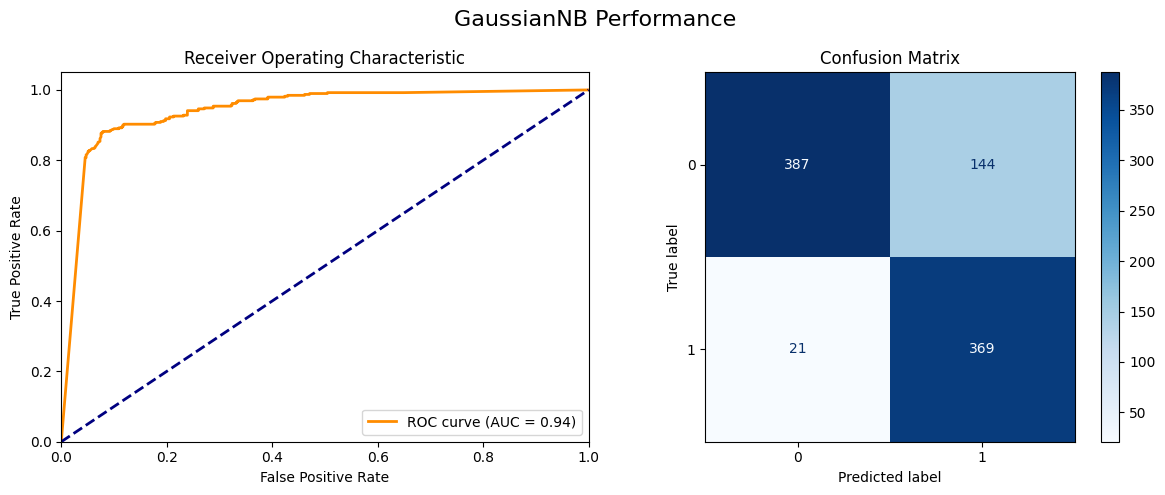
\includegraphics[width=0.8\textwidth]{images/naivebayes1.png}
\caption{ROC Curve and Confusion Matrix - Na\"ive Bayes GaussianNB}
\end{figure}

\begin{figure}[h!]
\centering
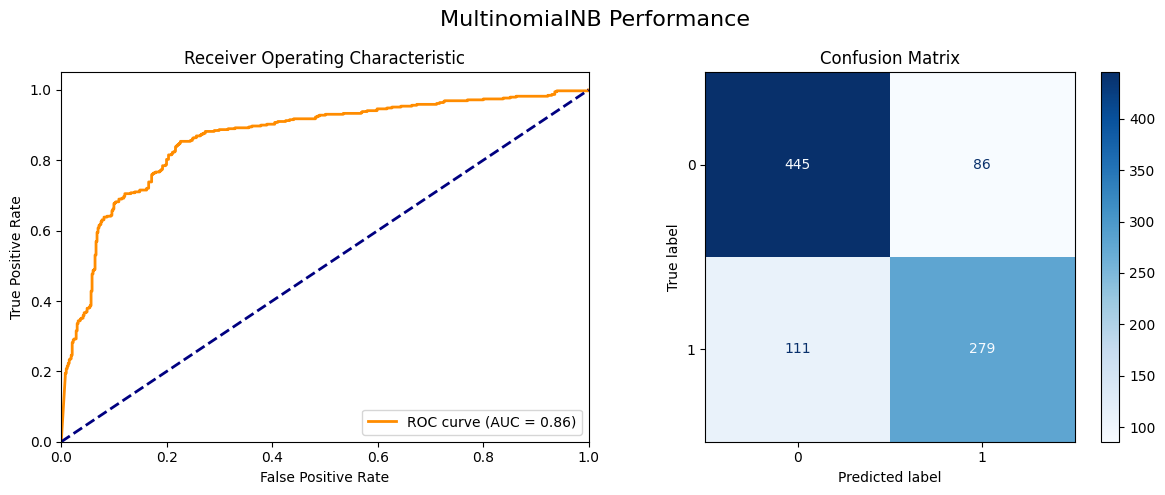
\includegraphics[width=0.8\textwidth]{images/naivebayes2.png}
\caption{ROC Curve and Confusion Matrix - Na\"ive Bayes MultinomialNB}
\end{figure}

\begin{figure}[h!]
\centering
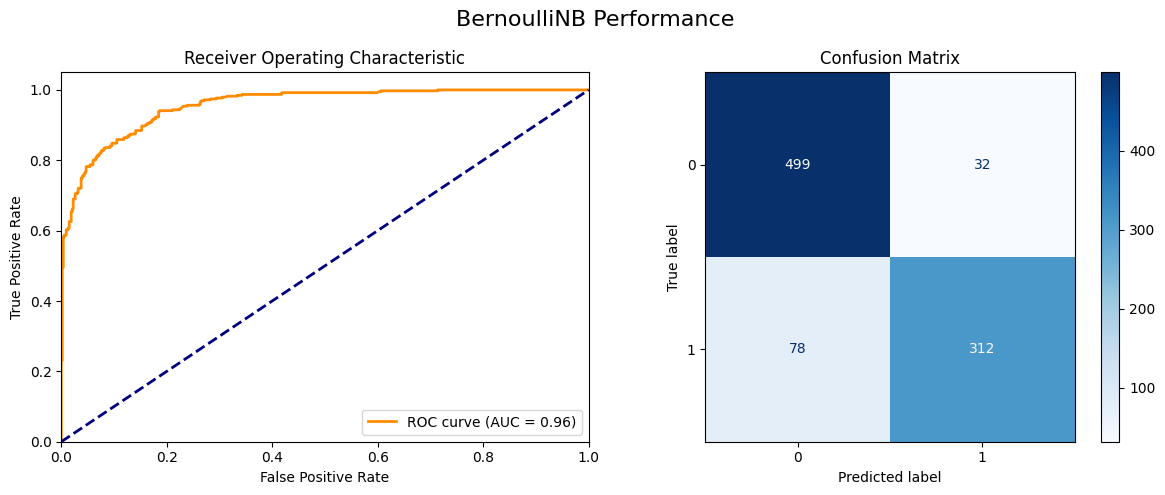
\includegraphics[width=0.8\textwidth]{images/naivebayes3.png}
\caption{ROC Curve and Confusion Matrix - Na\"ive Bayes BernoulliNB}
\end{figure}


\begin{figure}[h!]
\centering
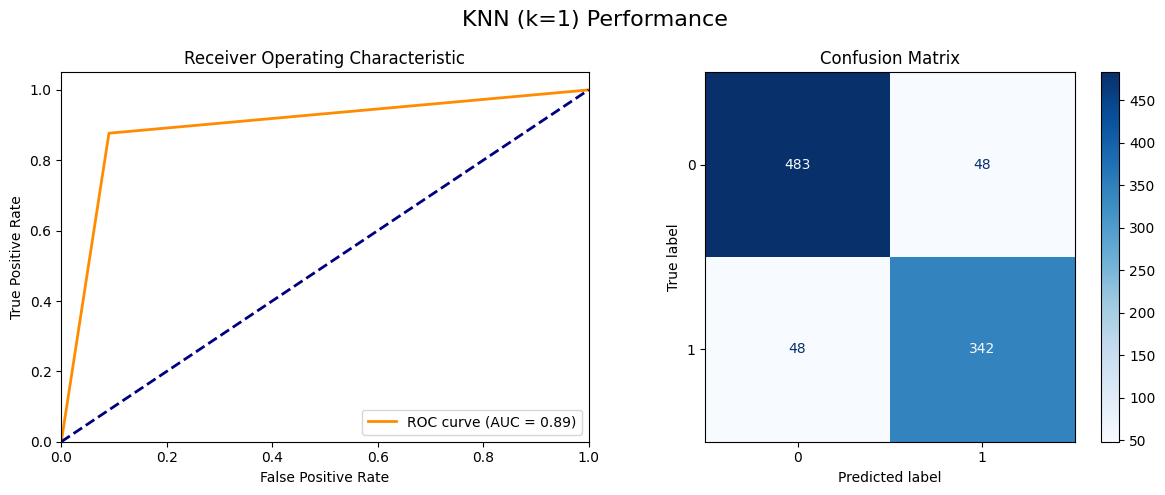
\includegraphics[width=0.8\textwidth]{images/knn1.png}
\caption{ROC Curve and Confusion Matrix - KNN (K=1)}
\end{figure}

\begin{figure}[h!]
\centering
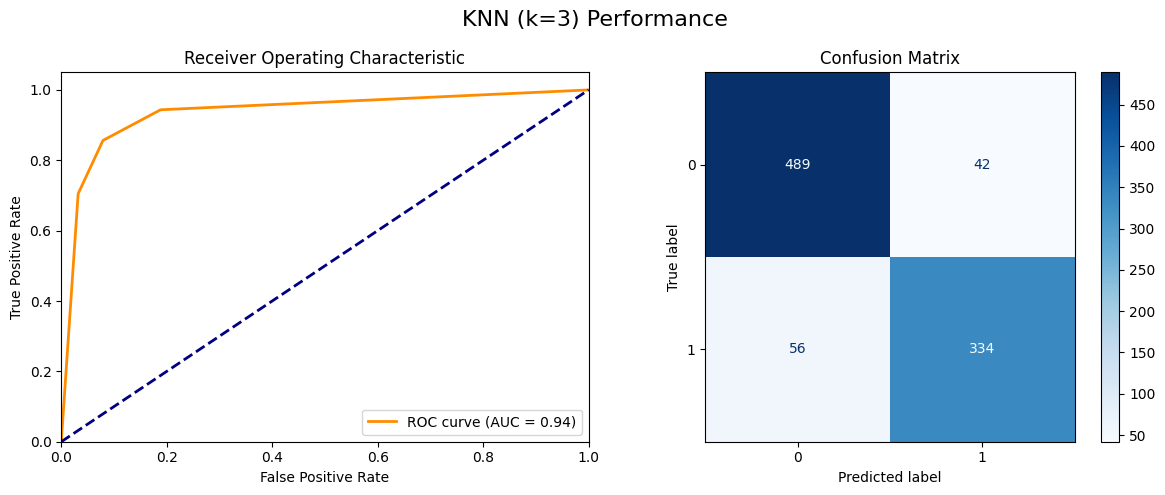
\includegraphics[width=0.8\textwidth]{images/knn2.png}
\caption{ROC Curve and Confusion Matrix - KNN (K=3)}
\end{figure}

\begin{figure}[h!]
\centering
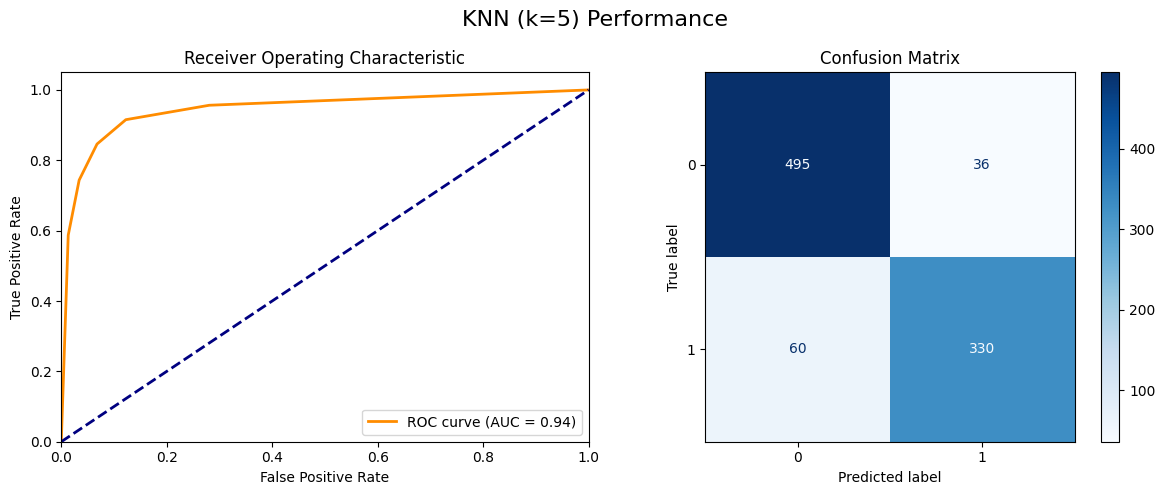
\includegraphics[width=0.8\textwidth]{images/knn3.png}
\caption{ROC Curve and Confusion Matrix - KNN (K=5)}
\end{figure}

\begin{figure}[h!]
\centering
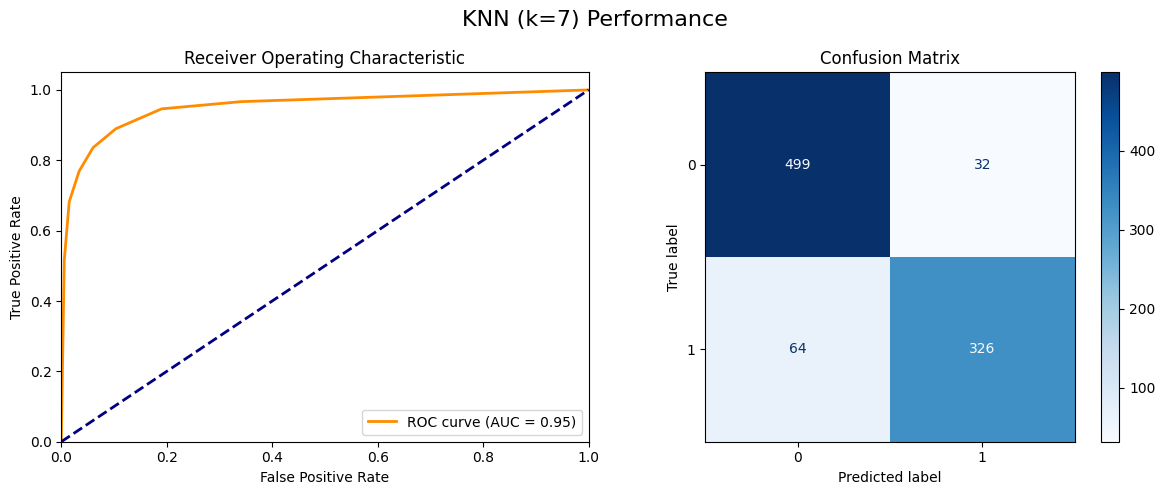
\includegraphics[width=0.8\textwidth]{images/knn4.png}
\caption{ROC Curve and Confusion Matrix - KNN (K=7)}
\end{figure}

\begin{figure}[h!]
\centering
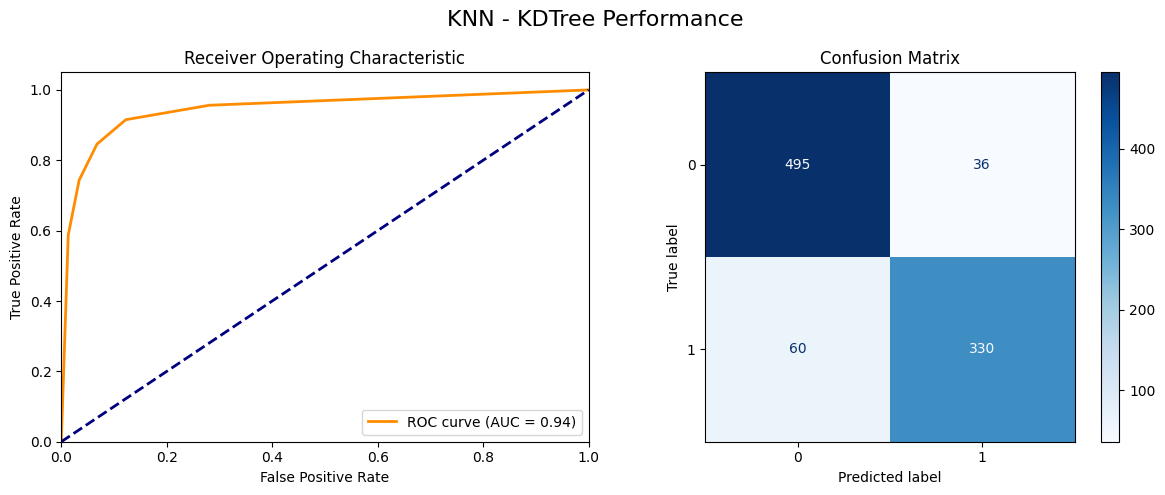
\includegraphics[width=0.8\textwidth]{images/knn5.png}
\caption{ROC Curve and Confusion Matrix - KNN (KDTree)}
\end{figure}

\begin{figure}[h!]
\centering
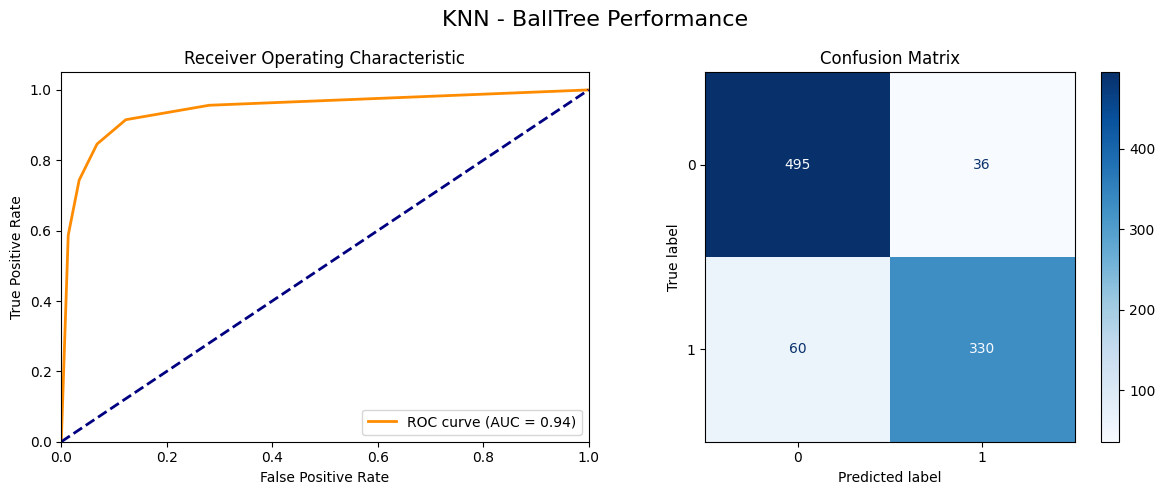
\includegraphics[width=0.8\textwidth]{images/knn6.png}
\caption{ROC Curve and Confusion Matrix - KNN (BallTree)}
\end{figure}

\begin{figure}[h!]
\centering
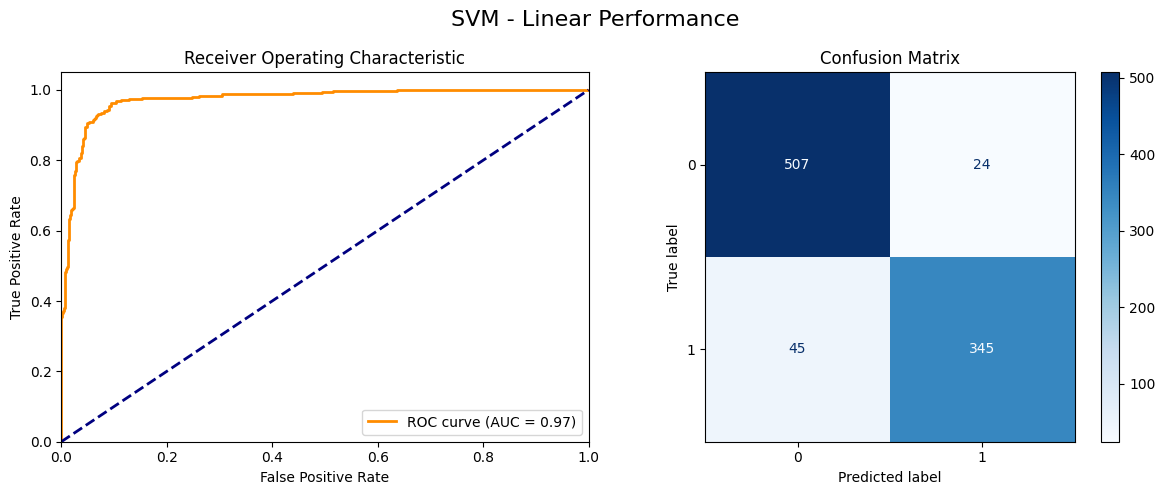
\includegraphics[width=0.8\textwidth]{images/svm1.png}
\caption{ROC Curve and Confusion Matrix - SVM Linear }
\end{figure}

\begin{figure}[h!]
\centering
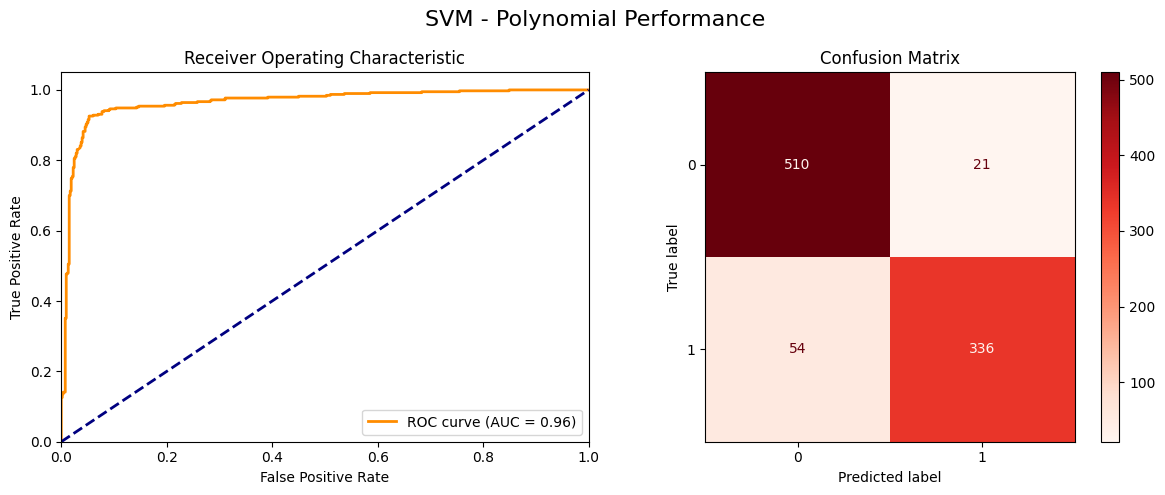
\includegraphics[width=0.8\textwidth]{images/svm2.png}
\caption{ROC Curve and Confusion Matrix - SVM Polynomial }
\end{figure}

\begin{figure}[h!]
\centering
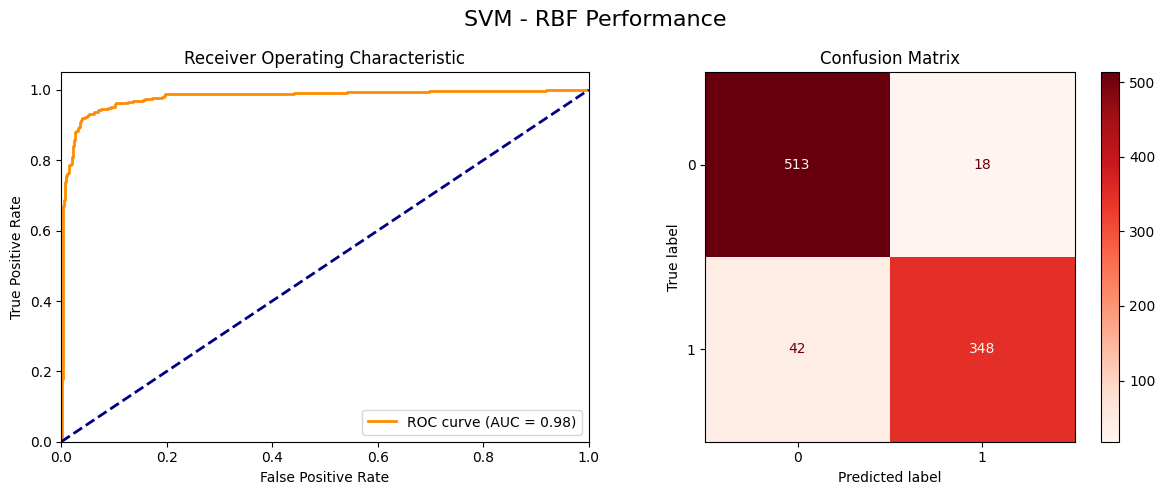
\includegraphics[width=0.8\textwidth]{images/svm3.png}
\caption{ROC Curve and Confusion Matrix - SVM RBF }
\end{figure}

\begin{figure}[h!]
\centering
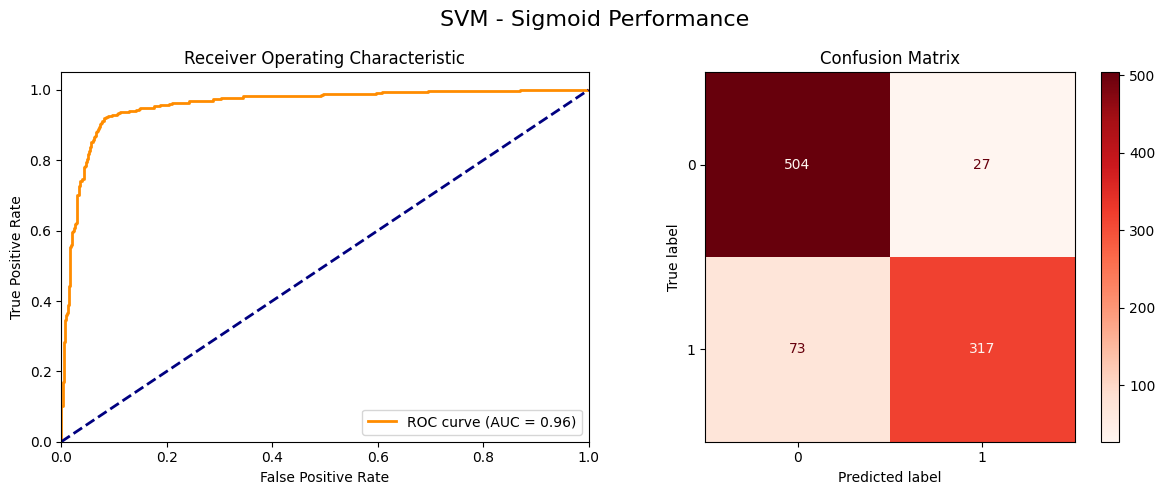
\includegraphics[width=0.8\textwidth]{images/svm4.png}
\caption{ROC Curve and Confusion Matrix - SVM Sigmoid }
\end{figure}


\clearpage

\section*{Results and Comparisons}

\subsection*{Table 1: Naïve Bayes Variant Comparison}
\begin{tabular}{|l|c|c|c|c|}
\hline
\textbf{Metric} & \textbf{Gaussian NB} & \textbf{Multinomial NB} & \textbf{Bernoulli NB} \\
\hline
Accuracy & 0.820847 & 0.786102 & 0.880565 \\
Precision & 0.719298 & 0.764384 & 0.906977 \\
Recall & 0.946154 & 0.715385 & 0.800000 \\
F1 Score & 0.817276 & 0.739073 & 0.850136 \\
\hline
\end{tabular}

\vspace{1em}

\subsection*{Table 2: KNN Performance for Different k}
\begin{tabular}{|c|c|c|c|c|}
\hline
\textbf{k} & \textbf{Accuracy} & \textbf{Precision} & \textbf{Recall} & \textbf{F1 Score} \\
\hline
1 & 0.895765 & 0.876923 & 0.876923 & 0.876923 \\
3 & 0.893594 & 0.888298 & 0.856140 & 0.872063 \\
5 & 0.895765 & 0.901639 & 0.846154 & 0.873016 \\
7 & 0.895765 & 0.910615 & 0.835897 & 0.871658 \\
\hline
\end{tabular}

\vspace{1em}

\subsection*{Table 3: KNN Comparison: KDTree vs BallTree}
\begin{tabular}{|l|c|c|}
\hline
\textbf{Metric} & \textbf{KDTree} & \textbf{BallTree} \\
\hline
Accuracy & 0.895765 & 0.895765 \\
Precision & 0.901639 & 0.901639 \\
Recall & 0.846154 & 0.846154 \\
F1 Score & 0.873016 & 0.873016 \\
Training Time (s) & 0.812832 & 0.808676 \\
\hline
\end{tabular}

\vspace{1em}

\subsection*{Table 4: SVM Performance with Different Kernels}
\begin{tabular}{|l|l|c|c|c|}
\hline
\textbf{Kernel} & \textbf{Hyperparameters} & \textbf{Accuracy} & \textbf{F1 Score} & \textbf{Train Time (s)} \\
\hline
Linear & C=1 & 0.925081 & 0.909091 & 2.467797 \\
Polynomial & C=1, degree=3, gamma=scale & 0.764387 & 0.629060 & 2.901383 \\
RBF & C=1, gamma=scale & 0.934853 & 0.920635 & 2.408404 \\
Sigmoid & C=1, gamma=scale & 0.889251 & 0.866492 & 1.829148 \\
\hline
\end{tabular}

\vspace{1em}

\subsection*{Table 5: K-Fold Cross-Validation Accuracy (K=5)}
\begin{tabular}{|l|c|c|c|}
\hline
\textbf{Fold} & \textbf{Naïve Bayes} & \textbf{KNN (k=5)} & \textbf{SVM (RBF)} \\
\hline
Fold 1 & 0.820847 & 0.895765 & 0.934853 \\
Fold 2 & 0.817391 & 0.904348 & 0.933696 \\
Fold 3 & 0.801087 & 0.929348 & 0.922826 \\
Fold 4 & 0.820652 & 0.903261 & 0.935870 \\
Fold 5 & 0.835870 & 0.909783 & 0.930435 \\
\textbf{Average} & 0.819169 & 0.908501 & 0.931536 \\
\hline
\end{tabular}

\section*{Conclusion}
In this experiment, we successfully implemented and evaluated three major classification algorithms: Na\"ive Bayes, K-Nearest Neighbors (KNN), and Support Vector Machine (SVM) on the Spambase dataset.  
Na\"ive Bayes was the fastest and performed well with Gaussian and Multinomial variants.  
KNN showed high accuracy with lower values of \( k \), but performance degraded as \( k \) increased.  
SVM, particularly with the RBF kernel, achieved the highest accuracy and F1-score overall.  
Standardization significantly improved KNN and SVM performance.  
ROC curves and confusion matrices highlighted SVM’s strong classification boundary.  
Thus, SVM with RBF kernel is most suitable for this spam classification task.


\end{document}
